\begin{refsection}[research/maruyama/group.bib]
\nocite{*}
\chapter{HPC Programming Framework Research Team}

\section{Members}

\begin{itemize}
  \item[] Naoya Maruyama (Team Leader)
  \item[] Motohiko Matsuda (Research Scientist)
  \item[] Shinichiro Takizawa (Research Scientist)
  \item[] Mohamed Wahib (Postdoctoral Researcher)
  \item[] Keisuke Fukuda (Research Associate)
  \item[] Koji Ueno (Student Trainee)
  \item[] An Huynh (Student Trainee)
  \item[] Satoshi Matsuoka (Senior Visiting Scientist)
  \item[] Tomoko Nakashima (Assistant)
  \item[] Aya Motohashi (Assistant)
\end{itemize}

Text for research Results and achievements. Journal-artcile~\cite{sample-journal}.
Conference-paper~\cite{sample-conference}.
Invited-talk~\cite{sample-invited}.

For cross referencing, use \verb|\locallabel| and \verb|\localref| to avoid conflicting names defined by other groups. For example, a figure can be referenced as Figure~\localref{fig:sample-label1}.

\begin{figure}
\centering
  
\includegraphics[width=0.5\textwidth,keepaspectratio,natwidth=193,natheight=40]
  {sample_division/sample_group/test1.png}
  \caption{Caption for a sample figure}
  \locallabel{fig:sample-label1}
\end{figure}

\section{Research Activities}

We develop high performance, highly productive software stacks that aim to simplify development of highly optimized, fault-tolerant computational science applications on current and future supercomputers, notably the K computer. Our current focus of work includes large-scale data processing, heterogeneous computing, and fault tolerance. A major ongoing project in our group will deliver a MapReduce runtime that is highly optimized for the intra- and inter-node architectures of the K computer as well as its peta-scale hierarchical storage systems. Another major project focuses on performance and productivity in large-scale heterogeneous systems. We also study high performance graph analytics on the K computer. Below is a brief summary of each project.

\section{Research Results and Achievements}

\subsection{KMR}
% Takizawa & Matsuda
\subsubsection{Improve locality when running MPI programs as MapReduce tasks}

Although MapReduce systems can allocate tasks to nodes where their inputs reside to increase data locality for improving performance, these systems only target on tasks implemented as serial programs and do not consider running tasks implemented as parallel programs using MPI as Map or Reduce task.
As many scientific applications are implemented using MPI and some application workflows form ensemble execution patterns of such MPI programs, the workflows can be implemented easily and efficient data access can be achieved if a MapReduce system can allocate tasks implemented using MPI so that it can exploit data locality in them.

We proposed an extension of the execution model of MapReduce to achieve high performance when running MPI programs as Map/Reduce tasks.%~\cite{takizawa_hpc151}.
We model data to be processed as Key-Value as the traditional MapReduce model.
However, to processing the data, we propose a new \verb|map| function which makes process groups where each process in a group has a key-value whose key is same as those of other processes in the group and applies a user-defined mapper, which is implemented using MPI, to the key-values using processes in each group.
Figure~\localref{fig:kmr-01} shows the execution flow.

\begin{figure}
\centering
  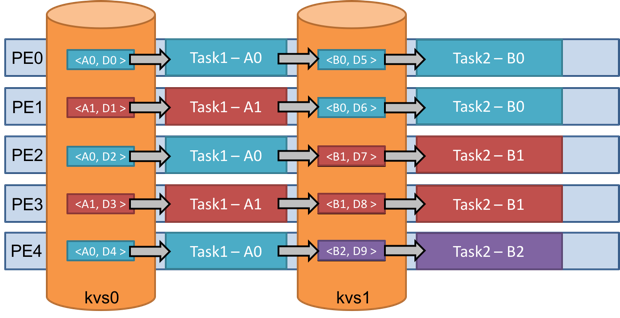
\includegraphics[width=0.5\textwidth,keepaspectratio,natwidth=193,natheight=40]
  {research/maruyama/lo01.png}
  \caption{Execution frow of MPI programm in MapReduce model}
  \locallabel{fig:kmr-01}
\end{figure}

To evaluate our proposal, we used $N \times N$ nodes of the K computer and compared performance of our method in which data access was performed locally and that of random data access.
We used a synthetic benchmark program where each node has an individual data and which iterates the following two computation; the first computation groups $N$ nodes in low direction and processes data on them, and the second groups $N$ nodes in column direction and processes data on them as showen in Figure~\localref{fig:kmr-02}.
The result is shown in Figure~\localref{fig:kmr-03}.
The horizontal axis is the amount of data on each node and the vertical axis is the relative performance of an iteration against random data access.
As can be seen from the figure, the performance of our proposal improve as the number of nodes and the amount of data increase.

\begin{figure}
\centering
  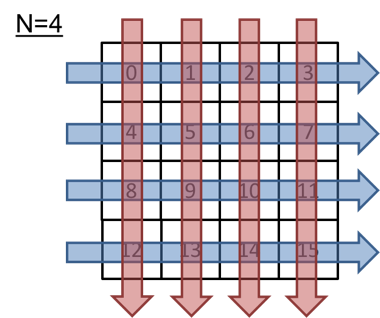
\includegraphics[width=0.5\textwidth,keepaspectratio,natwidth=193,natheight=40]
  {research/maruyama/lo02.png}
  \caption{Calculation pattern of the benchmark program}
  \locallabel{fig:kmr-02}
\end{figure}

\begin{figure}
\centering
  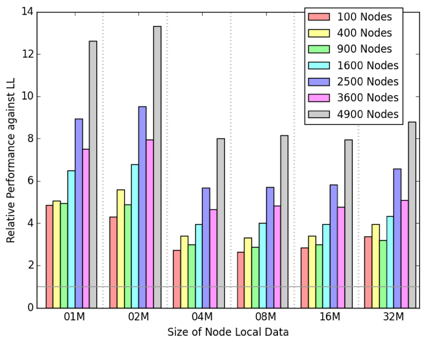
\includegraphics[width=0.5\textwidth,keepaspectratio,natwidth=193,natheight=40]
  {research/maruyama/lo03.png}
  \caption{Experimental results}
  \locallabel{fig:kmr-03}
\end{figure}


\subsubsection{Skew-tuned shuffling for load balancing for Reduce operation}

In a MapReduce program, the number of tasks in Map phase is defined by the number of split of the input data and that in Reduce phase is defined by the number of keys generated by the previous Map phase, and these numbers defines the maximum degree of parallelism of both phases.
Though the former can be defined by users when executing the program, users can not control the latter because it depends on patterns of applications and input data.
In contrast, as KMR statically defines number of processes used in both phase as the same value, we need to adopt load balancing techniques to average loads between processes in both phase.
Though balancing loads in Map phase can be left to users, a MapReduce system should support load balancing in Reduce phase as loads on processes heavily depend on the shuffle communication which is transparently performed by a system.

To balance loads on processes in Reduce phase, we proposed and implemented a shuffle algorithm that minimizes the skew of numbers of key-value pairs processed on each process~\cite{nishinaga_aics16}.
We referred to an existing algorithm LEEN and extended it as follows.
\begin{itemize}
\item used a distributed algorithm
\item reduce the number of search target keys (keys in key-value pairs) to reduce the cost of running the algorithm
\end{itemize}
We compared the performance of our method and that of using a shuffle that randomly assigned key-values to processes by using a benchmark program that implemented k-means on top of MapReduce.
As a result, time spent for executing Reduce task was reduced against the random shuffle as our proposal averaged the number of keys among processes.
On the other hand, we also confirmed that the overall execution time increased due to the large cost of running the algorithm.
We plan to reduce the algorithm execution cost as a future work.

\subsubsection{Visualize MapReduce task execution}

Widely used MapReduce systems, such as Apache Hadoop and Spark, have their own profiling and visualization tools to see the status of jobs.
They help users to look for performance bottlenecks, to do debug and to optimize their programs.
As KMR is implemented as one of an MPI library using the C language, we can use any profilers, such as gprof, Intel Vtune and FUJITSU profiler.
However, as they target on low level events, such as memory access and function calls, they are not suitable for profiling task level events in a MapReduce program.
We developed an event tracer for KMR that traced MapReduce operations, such as Map/Reduce tasks and Shuffle communication, and a visualization tool named KMRViz that displayed the traces in a GUI window.

The tracer traces KMR function calls and records times of start and end of a function and numbers of input and output key-value pairs of the function.
To eliminate IO overhead for writing records during a program execution, we implemented the tracer so that it recorded profiles in-memory while execution and wrote them to files at the end of the program execution.
Moreover, to eliminate the burden of using the tracer, we implemented it so that the tracer could be enabled just by setting an environment variable.
KMRViz receives trace files generated by the tracer and displays them in time series by each process as the Figure~\localref{fig:kmrviz}.
It is implemented using GTK+3 and users can zoom-in and out using mice and trackpads.

\begin{figure}
\centering
  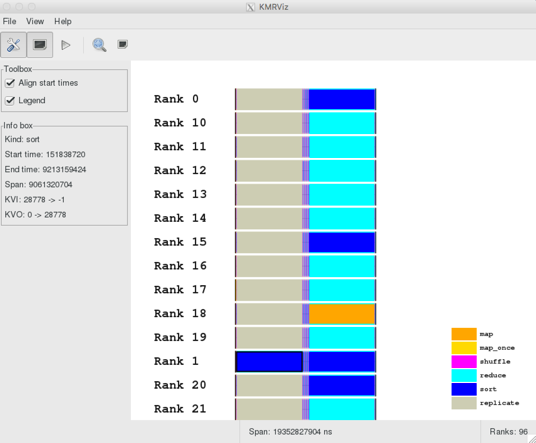
\includegraphics[width=0.5\textwidth,keepaspectratio,natwidth=193,natheight=40]
  {research/maruyama/kmrviz.png}
  \caption{Screenshot of KMRViz}
  \locallabel{fig:kmrviz}
\end{figure}


\subsubsection{Apache Spark on K computer}


\subsection{High Level Framework for High Performance AMR}
% Wahib

\subsection{High Performance Graph Analytics Study with Graph500}
% Maruyama

\section{Schedule and Future Plan}

\subsection{KMR}
% Takizawa & Matsuda

We plan to extend our first research activity (Improve locality when running MPI programs as MapReduce tasks) to improve the representation of programs.
Because the current version depends on key-value pairs as data exchanged between tasks as the usual MapReduce model but supports both serial and parallel MPI execution, we have to distinguish Map functions for these two cases and actually implemented them as different functions.
It is obviously redundant as their objective is the same; mapping data.
Moreover, users can not recognize the number of processes used in each MPI programs run as Map because they are unaware of locations of input key-value pairs and number of processes that hold the input key-value pairs.

To overcome these problems, we are developing a hybrid programming model of MPI message passing and MapReduce model.
In this model, we model data exchanged between tasks as multi-dimensional array which can be split to process each chunk depending on user perspectives at run time.
The location of chunks of the multi-dimensional array is also changeable at run time.
A Map function in this model applies a user-defined function to each chunk of the multi-dimensional array using processes that hold the data.
We are developing the model and applying it to application workflows that perform ensemble simulations.

As for KMRViz, we plan to support more KMR operations to trace and visualize them.

\subsection{High Level Framework for High Performance AMR}
% Wahib

\subsection{High Performance Graph Analytics Study with Graph500}
% Maruyama

%%% DO NOT EDIT BELOW

\section{Publications}

%\printbibliography[keyword=journal, heading=subbibliography, title={Journal Articles}, prefixnumbers={1-}, resetnumbers=true]
%\printbibliography[keyword=proceedings, heading=subbibliography, title={Conference Papers}, prefixnumbers={2-}, resetnumbers=true]
%\printbibliography[keyword=invited, heading=subbibliography, title={Invited Talks}, prefixnumbers={3-}, resetnumbers=true]
%\printbibliography[keyword=poster, heading=subbibliography, title={Posters and Presentations}, prefixnumbers={4-}, resetnumbers=true]
%\printbibliography[keyword=deliverable, heading=subbibliography, title={Patents and Deliverables}, prefixnumbers={5-}, resetnumbers=true]

\printbibliography[keyword=journal, heading=subbibliography, title={Journal Articles}, resetnumbers=true]
\printbibliography[keyword=proceedings, heading=subbibliography, title={Conference Papers}]
\printbibliography[keyword=invited, heading=subbibliography, title={Invited Talks}]
\printbibliography[keyword=poster, heading=subbibliography, title={Posters and Presentations}]
\printbibliography[keyword=deliverable, heading=subbibliography, title={Patents and Deliverables}]

\end{refsection}
